\documentclass[final,dvipdfmx]{beamer}
\mode<presentation> {
  \usetheme{Berlin}
}
\usepackage{indentfirst}
\usepackage{ulem}
\usepackage{tasks}

\usepackage[orientation=portrait,size=a0,scale=1.4,debug]{beamerposter}
\usepackage[japanese]{babel}

\usepackage{multicol}

\usepackage{ascmac}


\begin{document}

\begin{minipage}[]{0.88\columnwidth}
	\vskip\baselineskip
	\Huge オープンソース開発プロセスの要素を導入した\\サーバ構築演習の授業設計と試験的評価 \\[5mm]
	\Large 大森裕介 (公立千歳科学技術大学理工学部/情報システム工学科/深町研究室)
\end{minipage}
\begin{minipage}[]{0.11\columnwidth}
	\begin{figure}\centering
		
\includegraphics[width=\columnwidth]{img/cist.png}
	\end{figure}
\end{minipage}\\[2mm]

\bigskip

\begin{columns}[T]
	\begin{column}{.49\linewidth}
		\begin{block}{背景}
			\textbf{教育手法} 近年,日本ではアクティブラーニング(AL)などを用いて,世界で求められている人材育成に取り組んでいる.
			\begin{columns}
				\begin{column}{0.48\textwidth}
					\textbf{目標} 学生が批判的な思考や学びかたの学習,異質な集団での問題解決能力の習得を目指している.
				\end{column}
				\begin{column}{0.01\textwidth} 
					\textbf{\Rightarrow}
				\end{column} 
				\begin{column}{0.48\textwidth}
					\textbf{課題} 学生が安易に回答を要求,派生知識に無関心,表面的な議論,認知プロセスの外化をしないこと\\
					\footnotesize{\textreferencemark 認知プロセスの外化:問題解決のために知識を使う,人に話す,書く,発表すること}
				\end{column}
			\end{columns}
						
			\vskip\baselineskip
						      
			\textbf{情報教育} 日本の教育では積極的にIT技術者の育成を行っている.大学教育では,実践的な技術者育成も重要視されており,その技術者像や技術者教育の到達目標や評価方法の提言もされている.
		\end{block}
				
		\begin{block}{目的}
			\vskip.5\baselineskip
			
			
			\begin{columns}
				\begin{column}{0.28\textwidth}
					\textbf{学習} 発展的なIT知識や実践的な学習
				\end{column}
				\begin{column}{0.01\textwidth} 
					\textbf{+}
				\end{column} 
				\begin{column}{0.68\textwidth}
					\textbf{姿勢} 社会で求められるIT人材の開発姿勢や主体的な知識習得,実践的な能力習得を身につける意識
				\end{column}
			\end{columns}
			
			
			\vskip.5\baselineskip
			
			\begin{shadebox}
				\textbf{サーバ構築演習という実践的な理工学部3年の選択授業を検証フィールドとし,オープンソース(OSS)開発プロセスの要素を取り入れた授業設計の有用性を評価する.}
			\end{shadebox}
			\vskip.5\baselineskip
			
			\begin{columns}
				\begin{column}{0.48\textwidth}
					\vskip.5\baselineskip
					\textbf{OSS開発プロセスとは},オープンソースソフトウェア開発を行う過程である.OSSはソースコードが公開されており,自由な利用,再配布を認めている.OSSの開発の多くは,無報酬で自発的に参加する世界中の開発者を中心として行われている.
				\end{column}
				\begin{column}{0.01\textwidth} 
					\textbf{\Rightarrow}
				\end{column} 
				\begin{column}{0.48\textwidth}
					\textbf{導入する要素}
					\begin{itemize} 
						\item 非同期なコミュニケーション 
						\item 知識の集約,共有 
						\item 情報の妥当性を評価 
						\item 認知プロセスの外化 
						\item 異質な集団でのコミュニケーション 
					\end{itemize} 
				\end{column}
			\end{columns}
						    
		\end{block}
				
		\begin{block}{方法}
			
			\begin{screen}
				\textbf{\large{姿勢}}\,
				\vskip.5\baselineskip
				IT業界やOSS活動で用いられているGitHubや技術ブログを用いた.
				
				\begin{table}[H]
					\caption{利用したもの}
					\label{tab:yakudatu}
					\centering
					\begin{tabular}{|c|c|c|} \hline
						名前        & 理由                                                                       & 利用期間       \\ \hline
						GitHub          & \begin{tabular}{l}$\bullet$学生同士の非同期コミュニケーション\\$\bullet$知識の集約の場\\$\bullet$学習プロセスの可視化\\$\bullet$異質な集団に近づけ,情報の妥当性を評価\end{tabular} & 検証全体 \\ \hline
						技術ブログ & \begin{tabular}{c}外部に対して認知プロセスの外化\end{tabular} & 検証後半以降 \\ \hline
					\end{tabular}
				\end{table}
				
			\end{screen}
			
			\normalsize
			   
			% \hrulefill\\[9mm]
			\begin{screen}
				   
				\textbf{\large{学習}}\,
				\vskip.5\baselineskip
				本検証は全15回の演習授業で行った.\textbf{授業構成は前半と後半で分かれる.}
				\vskip.5\baselineskip
				\textbf{前半}\,\\多くの学生はサーバ構築未経験者のため,資料とワークシート,サーバ構築演習支援ツールを用いて,仮想サーバ上にLAMP構成のWEBアプリケーション構築を行い基礎から学習
				\vskip.5\baselineskip
				\textbf{後半}\,\\「なんらかの連携をするシステムを構築する」という自由な課題
				
				\begin{table}[!ht]
					\caption{全15回の授業計画}
					\label{tab:zyugyouplan}
					\centering
					\begin{tabular}{|l|l|l|l|l|}
						\hline
						授業回数    & 第1回                                     & 第2回〜第6回            & 第7回         & 第8回         \\ \hline
						授業形態    & オンライン                             & オンライン              & オンライン & オンライン \\ \hline
						内容          & \begin{tabular}{c}調べ学習\end{tabular} & \begin{tabular}{c}LAMP環境\\構築演習\end{tabular} & \begin{tabular}{c}LAMP環境\\構築演習の\\口頭試問\end{tabular} & \begin{tabular}{c}E-learningの\\テスト\end{tabular} \\ \hline
						授業外学習 & E-learning                                  & E-learning               & E-learning      & 指示なし    \\ \hline
						                        
						授業回数 & 第9回〜第14回 & 第15回 & \multicolumn{2}{|c|}{} \\ \hline
						授業形態 & オンライン & 対面 & \multicolumn{2}{|c|}{} \\ \hline
						内容 & \begin{tabular}{c}自由課題\end{tabular} & \begin{tabular}{c}自由課題の\\成果発表\end{tabular} & \multicolumn{2}{|c|}{}\\ \hline
						授業外学習 & 指示なし & 指示なし & \multicolumn{2}{|c|}{} \\ \hline
					\end{tabular}
				\end{table}
				
				\begin{table}[H]
					\caption{利用したもの}
					\label{tab:yakudatu}
					\centering
					\begin{tabular}{|c|c|c|} \hline
						名前           & 理由                                                                      & 利用期間     \\ \hline
						仮想サーバ    & 演習環境を提供するため                                           & 前半,後半  \\ \hline
						ワークシート & 演習の内容を示すため                                              & 前半           \\ \hline
						演習資料       & \begin{tabular}{l}$\bullet$多くの学生はサーバ構築未経験者のため\\$\bullet$派生知識に関心を促すため\end{tabular} & 前半 \\ \hline
						支援ツール    & \begin{tabular}{c}自己解決を促すため\end{tabular}                  & 前半           \\ \hline
					\end{tabular}
				\end{table}
				
			\end{screen}
			
		\end{block}
				
				    
	\end{column}
	\begin{column}{.49\linewidth}
		\begin{block}{評価・考察}
			
			\begin{screen}
				\textbf{\large{前半の演習が与えた主体的な学習効果}}\,
				\vskip.5\baselineskip
				前半の演習を行い,\textbf{3割以上の学生がサーバ構築に興味(注意)を持ち,将来役に立つ(関連性)と思い,サーバ構築に自信(自信)を持つ}ように変化
				
				\begin{columns}
					\begin{column}{0.6\textwidth}
						\begin{table}[H]
							\caption{ARCSモデルのアンケート結果(n=25)}
							\label{tab:yakudatu}
							\centering
							\begin{tabular}{|c|c|c|c|} \hline
								項目  & 向上      & 変化なし   & 低下       \\ \hline
								注意    & 9人(36\%)  &  15人(60\%) & 1人(4\%)    \\ \hline
								関連性 & 8人(32\%)  &  10人(40\%) & 7人(28\%)   \\ \hline
								自信    & 13人(52\%) & 10人(40\%)    & 2人(8\%)  \\ \hline
							\end{tabular}
						\end{table}
					\end{column}
					\begin{column}{0.4\textwidth}
						\textbf{変化の要因}
						\begin{itemize}
							\item 習得済みの知識との関連性を理解
							\item 周辺知識を学習
							\item 前半の課題が完了
						\end{itemize}
					\end{column}
				\end{columns}
				
				
			\end{screen}
			
			\normalsize
			
			\begin{screen}
				   
				\textbf{\large{同期,非同期なコニュニケーションでの積極性などの違い}}\,
				\vskip.5\baselineskip
				
				\begin{columns}
					\begin{column}{0.48\textwidth}
						\quad\textbf{非同期なコミュニケーション}\\ \quad\small{本検証のGitHubのコメント}
					\end{column}
					\begin{column}{0.01\textwidth} 
						\textbf{$<$}
					\end{column} 
					\begin{column}{0.48\textwidth}
						\textbf{同期的なコミュニケーション}\\ \small{本検証以外のグループワーク}
					\end{column}
				\end{columns}
				
				\vskip.5\baselineskip
				
							
				\begin{table}[H]
					\caption{非同期なコミュニケーションと同期的なコミュニケーションの特性}
					\label{tab:hidouki_douki}
					\centering
					\begin{tabular}{|c|c|c|c|c|} \hline
						\begin{tabular}{c}\end{tabular} & \begin{tabular}{c}積極性\end{tabular} & \begin{tabular}{c}難易度\end{tabular} & \begin{tabular}{c}時間\end{tabular} & \begin{tabular}{c}抵抗の有無\end{tabular}\\ \hline
						
						\begin{tabular}{c}同期的な  \\コミュニケーション\end{tabular} & \begin{tabular}{c}高い\end{tabular} & \begin{tabular}{c}低い\end{tabular} & \begin{tabular}{c}短い\end{tabular} & \begin{tabular}{c}ない\end{tabular}\\ \hline
						\begin{tabular}{c}非同期な  \\コミュニケーション\end{tabular} & \begin{tabular}{c}低い\end{tabular} & \begin{tabular}{c}高い\end{tabular} & \begin{tabular}{c}長い\end{tabular} & \begin{tabular}{c}ない\end{tabular}\\ \hline
					\end{tabular}
				\end{table}
				
				
				\footnotesize{\textreferencemark それぞれのコミュニケーションの「学生の他者貢献に対する積極性」,「学生が感じるコミュニケーションの難易度」,「コミュニケーションを行い問題解決するまでの時間」,「学生が発言することに対して抵抗があるか」について示した.}
				\\
				\footnotesize{\textreferencemark \textbf{21名(84\%)}の学生は\textbf{グループワーク}の方が積極的に発言できたと回答.}
				
				\normalsize
			\end{screen}
			\begin{screen}
				\textbf{\large{支援ツールについて}}
				\vskip.5\baselineskip
				\textbf{12名(48\%)}の学生が「\textbf{役に立った}」と回答
			\end{screen}
			
			\begin{screen}
				\textbf{\large{GitHubのコメント履歴}}\,
				\vskip.5\baselineskip
				\begin{itemize}
					\item  一部の投稿で質問するべき問題やエラー情報が整理されておらず解決までに\textbf{時間かかる}ことがあった
					\item \textbf{演習を順調に進める学生は他者にコメントしない}傾向
				\end{itemize}
			\end{screen}
			\begin{screen}
				\textbf{\large{技術ブログ}}\,
				\vskip.5\baselineskip
				教員からの働きかけにより,\textbf{3名}の学生が技術ブログを執筆
			\end{screen}
			\begin{screen}
				\textbf{\large{インタビュー}}\,
				\vskip.5\baselineskip
				4名の学生の特性に関して調査
				
				   
				
				\vskip.5\baselineskip
				
				\begin{columns}
					\begin{column}{0.5\textwidth}
						\begin{itemize}
							\item \textbf{学内外かかわらず主体的に課外活動に取り組む学生}\\$\bullet$新しいことへの\textbf{挑戦を苦痛に感じていない}\\$\bullet$\textbf{技術ブログを執筆}
						\end{itemize}
					\end{column}
					\begin{column}{0.5\textwidth}
						\begin{itemize} 
							\item \textbf{課外活動に消極的(苦痛)な学生}\\$\bullet$\textbf{主体的に学ぶことが苦痛}\\$\bullet$\textbf{能動的に課題に取り組んでいない\\$\bullet$\textbf{課題を完了することが目的}}\\$\bullet$\textbf{課題に時間がかかると苦痛}
						\end{itemize}
					\end{column} 
				\end{columns}
				
			\end{screen} 
			
			\begin{screen}
				\textbf{\large{後半の課題}}
				\begin{itemize}
					\item 作成したアプリケーションについての説明資料とアプリケーションのソースコードをGitHubで公開した学生
					\item \textbf{本検証内で執筆した学生の技術ブログを参考に後半の課題に取り組んだ学生}
				\end{itemize} 
				       
			\end{screen}
						
		\end{block}
				
		\begin{block}{議論}
			
			\begin{columns}
				
				\begin{column}{0.43\textwidth}
					\vskip.5\baselineskip
						\textbf{意欲的,主体的な学生}
						      \begin{itemize}
						      	\item 授業で学んだ知識や自身で学んだ知識を外部に知識を公開
						      	\item 外部の集団と交流
						      \end{itemize}
            \vskip.5\baselineskip
						\textbf{消極的な学生}
						      \begin{itemize}
						      	\item 課外活動や授業に消極的
						      	\item 面白そうな情報,同じ世代がまとめた情報から学習
						      	\item 少しづつ意欲的に変化
						      \end{itemize}
					
					\vskip.5\baselineskip
					
					$\Rightarrow$ 意欲的な学生が,楽しみながら意欲的に纏めた体系的な情報が,他の学生に良い影響を与えることにつながると考えられる.
					   
				\end{column}
				\begin{column}{0.55\textwidth}
					\begin{figure}[H]
						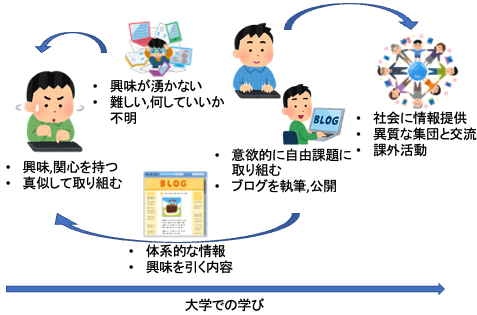
\includegraphics[width=220mm]{img/OSS_pr.png}
						\caption{意欲的な学生と意欲的でない学生の学び}
					\end{figure}
				\end{column}
			\end{columns}
			
					
		\end{block}
		
		
				    
	\end{column}
\end{columns}

\end{document}